\RequirePackage[2020-02-02]{latexrelease}
\documentclass[twocolumn]{revtex4}

\usepackage[utf8]{inputenc}
\usepackage{lmodern}
\usepackage[T1]{fontenc}
\usepackage{mathtools}
\usepackage{float}
\usepackage{csvsimple}
\providecommand{\abs}[1]{\lvert#1\rvert}
\usepackage{braket}
\providecommand{\eq}[2]{
    \begin{equation}
        #2
    \label{eq:#1}
    \end{equation}
}
\providecommand{\eqgat}[2]{
    \begin{gather}
        #2
    \label{eq:#1}
    \end{gather}
}
\usepackage{amsmath}
\usepackage{amsfonts}
\DeclareMathOperator{\calA}{\mathcal{A}}
\DeclareMathOperator{\calB}{\mathcal{B}}
\DeclareMathOperator{\calH}{\mathcal{H}}
\DeclareMathOperator{\calL}{\mathcal{L}}
\DeclareMathOperator{\tr}{tr}
\usepackage{fancyhdr}
\usepackage{wrapfig}
\usepackage{graphicx}
% \usepackage[hidelinks]{hyperref}



\begin{document}


\pagestyle{fancy}
\lhead{\bf Entanglement Entropy and Holography}
\rhead{Ferran Rodríguez Mascaró}
\lfoot{Treball de Fi de Grau}
\rfoot{Barcelona, January 2023}


\title{Entanglement Entropy and Holography}
\author{Author: Ferran Rodríguez Mascaró}
\email{ferran.r.m11@gmail.com} %optional
\affiliation{Facultat de F\'{\i}sica, Universitat de Barcelona, Diagonal 645, 08028 Barcelona, Spain.}
\author{Advisor: Pablo Bueno Gómez}
%\date{\today}


\begin{abstract}
    {\bf Abstract:} The AdS/CFT correspondence, also called Holography, is a duality relating quantum field theory and gravity, in particular conformal field theory and anti-de Sitter spacetime-time gravities. It describes how quantities from each of these theories, the so-called holographic dictionary, can be studied one through the other. One of the most important magnitudes of the holographic dictionary is the entanglement entropy of a region, that measures the degree of quantum entanglement between this region and its surroundings. In this work it is introduced the basics of holography, especially applied to entanglement entropy, demonstrating some important properties and fascinating achievements of the theory, as the equivalence of the Ryu-Takayanagi formula with the Bekenstein-Hawking black hole entropy formula, the fulfilment of the strong subadditivity property or the duality between entanglement entropy and the Einstein field equations.
\end{abstract}


\maketitle


\section{Introduction} \label{s:Intro}


\newpage


\section{Holography and AdS/CFT}


\subsection{The Holographic Principle} \label{ss:Holography}

Having a finite space region, one can imagine matter being added into it and hence the entropy of it also increasing. But there is a limit of the amount of matter that can be introduced to the region, corresponding to the moment a black hole is formed. Therefore, it appears to be also a cut-off of the entropy that the region can have equal to the entropy of a black hole filling it \cite{t_hooft_dimensional_2009}. The entropy of a black hole only depends on its area \cite{bekenstein_black_1973}, so the maximum entropy that a region could contain will also be only proportional to its area.

The covariant entropy bound \cite{bousso_covariant_1999} is conjectured as the representation of the universal law, in a four-dimensional spacetime on which Einstein equations are satisfied, in which the entropy of a system is bounded by its area.

This bound implies that the degrees of freedom inside some region grows with the area of the boundary and not as the volume of the region. This behaviour leads to the \textit{holographic principle}, which states that in a quantum gravity theory all the physics phenomena within some volume can be described in terms of a theory on the boundary of the area of the volume, which must has less than one degree of freedom per Planck area \cite{t_hooft_dimensional_2009}.


\subsection{AdS/CFT Correspondence} \label{ss:AdS/CFT}

The \textit{AdS/CFT correspondence}, simply called \textit{holography} or \textit{gauge/gravity correspondence} \cite{ramallo_introduction_2013}, is a realization of the holographic principle.

The AdS/CFT correspondence is the complete physical equivalence between quantum gravity theories living in anti-de Sitter spacetimes and certain types of conformal (with conformal symmetry) quantum field theories (QFT) living in the anti-de Sitter boundary (the \textit{conformal boundary}).

It allows us to study aspects of each of these theories through the other. The so-called \textit{holographic dictionary} relates quantities (observables) between the anti-de Sitter (AdS) theories and the Conformal Filed Theories (CFTs). % \cite{kaplan_lectures_nodate}

An anti-de Sitter spacetime is a maximally symmetric spacetime with negative curvature, solution to Einstein field equations with a negative cosmological constant. The metric of an AdS spacetime of $D=d+1$ dimensions using the coordinate system of the Poincaré patch is
\eq{AdS_PP-metric}{
    ds_{AdS_D}^2 = \frac{1}{z^2} \left( -dt^2 + dz^2 + \sum_{i=1}^{d-1} dx_i^2 \right) \ ,
}
\cite{kaplan_lectures_nodate} with the time and space-related dimensions $t , x_i \in (-\infty,+\infty)$ and an extra dimension $z \in (0,+\infty)$. Fixing the coordinate $z$, one creates $d$-dimensional spacetime surfaces 'weighted' by the factor $\frac{1}{z^2}$. At constant time, these lattices are hyperbolic spaces of negative curvature, conformally equivalent to Minkowski spacetimes when $z \to 0$ \cite{}.

AdS$_{d+1}$ spacetimes (the subscript expresses de dimensions of the theory) can be represented as cylinders where every slice corresponds to a constant time and where the extra dimension $z$ is radial component to the center of the cylinder \cite{}. Each slice would have a $d$-dimensional boundary $\partial$AdS$_{d+1}$ where the CFT$_d$ will live (Fig.~\ref{fig:AdS}).

\begin{wrapfigure}{r}{0.2\textwidth}
    \centering
    
\includegraphics[width=0.2\textwidth]{../Imatges/empty.png}
\caption{Cylindrical representation of an AdS$_3$ spacetime. It is represented a conformal boundary corresponding to a CFT$_2$.}
\label{fig:AdS}
\end{wrapfigure}

Conformal Field Theories are the type of QFT that are invariant under conformal coordinate transfromations, which leave the metric invariant under scale changes preserving the angles between vectors \cite{ginsparg_applied_1988}. One notices that the Poincaré group is a subgroup of the conformal group. The number of generators of a $d$-dimensional CFT coincides with the number of isometries of a $d+1$-dimensional AdS spacetime \cite{}.

The gauge/gravity correspondence is valid independently of the degree of gravitational coupling. A very gravitational coupled QFT is dual to a classical gravitational theory (Eisntein equations). In this case, it is possible to explain gravitational fenomena by quantum properties, and vice versa, using the holographic dictionary. For example, an empty AdS spacetime with no matter is dual to an empty CFT, and an AdS spacetime with a black hole inside corresponds to a thermalized CFT.


\section{Entanglement Entropy in CFT} \label{s:EE_CFT}

When two quantum systems enter into temporary physical interaction, they can no longer be described in the same way after a time of mutual influence \cite{schrodinger_discussion_1935}. One can no longer describe neither of those systems independently without losing global information, because the state of each system knows is influenced and correlated by the other system. This is the so-called \textit{quantum entanglement}.

The \textit{entanglement entropy} is a measure of the degree of quantum entanglement between the two subsystems composing a full quantum system \cite{nishioka_entanglement_2018}. It is defined by the von Neumann entropy of the reduced density matrix $\rho_A$ of one of the subsystems as
\eq{EE}{
    S_{EE}(A) = - \tr_A ( \rho_A \log \rho_A ) \ ,
}
being $\rho_A = \tr_B \ket{\Psi}\bra{\Psi}$. If $\rho_A$ is diagonalized ($\rho_A = \sum_i \lambda_i \ket{i}\bra{i}$), then the entanglement entropy would take the simplified form $S_{EE} = - \sum_i \lambda_i \log \lambda_i$.

The von Neumann entropy is always positive, and is null for a pure state (no entanglement).

For a QFT living in a Minkowski spacetime, one can define operator algebras that define spacetime regions. Discretizing the lattice, a density matrix is associated to the region that only depends on its algebra and its surroundings. From this density matrix, an entanglement entropy can be defined. The entanglement entropy will diverge, since the region is separed from its vicinity by a zero-dimensional boundary.

The general expression of the entanglement entropy for a $d$-dimensional QFT is
\eqgat{EE}{
    S_{QFT_d} = c_{d-2} \left( \frac{H}{\delta} \right) ^{d-2} + c_{d-1} \left( \frac{H}{\delta} \right) ^{d-4} + ... + \nonumber \\
    + \begin{dcases}
        c_1 \frac{H}{\delta} + (-1)^{\frac{d-1}{2}} s_{\text{univ}}
        \qquad \qquad \qquad \quad \ \text{for odd } d \\
        c_2 \left ( \frac{H}{\delta} \right ) + (-1)^{\frac{d-2}{2}} s_{\text{univ}} \log \left ( \frac{H}{\delta} \right ) + c_0
        \quad \text{for even } d
    \end{dcases} \ ,
}
\cite{nishioka_entanglement_2018} in which $H$ is the characteristic length of the region studied, $\delta$ is the ultraviolet cut-off, $c_i$ are coefficients that are non-universal (not well-defined in the continuum, dependent on the definition of $\delta$) and local, and $s_{\text{univ}}$ are universal coefficients that contain information about the corresponding QFT.


\section{Holographic Entanglement Entropy} \label{s:EE_Holo}


\subsection{Ryu-Takayanagui formula} \label{ss:R-T}

Generally, it is difficult to compute the entanglement entropy of a region, but it is sceptionally easy to do so using the AdS/CFT correspondence, being an entrance in the holographic dictionary. In the holographic context, an essentially quantum quantity such as entanglement entropy is found from areas within an AdS spacetime determined by its metric.

In a ($d+1$)-dimensional AdS spacetime, being $\calA$ a region of a $d$-dimensional Minkowski spacetime slice formed from fixing $z$ as $z=\delta \ll 1$, the entanglement entropy of a $d$-dimensional CFT on this Minkowski spacetime will be expressed by the so-called Ryu-Takayanagi formula:
\eq{EE_RT}{
    S_{\calA} = \frac{ \text{Area}(\gamma_{\calA}) }{ 4 G_{d+1} } \ ,
}
\cite{ryu_holographic_2008} where $\gamma_{\calA}$ is the surface of minimal area on the whole AdS spacetime connected to the ($d-1$)-dimensional boundary $\partial \calA$ of the region $\calA$, and $G_{d+1}$ is the ($d+1$)-dimensional Newton constant (represented in Fig.~\ref{fig:EE_AdS-CFT}).

The area of $\gamma_{\calA}$ is obtained by
\eq{EE_RT-area}{
    \text{Area}(\gamma_{\calA}) = \int_{\gamma_{\calA}} \sqrt{h} \ d^{d}y \ ,
}
where $y$ are the $d$ coordinates that represent surface $\gamma_{\calA}$ and $h$ is the determinant of the metric $h_{ij} = \frac{\partial x^\mu}{\partial y^i} \frac{\partial x^\nu}{\partial y^j} g_{\mu\nu}$ induced on the surface by the surrounding spacetime.

\begin{wrapfigure}{r}{0.25\textwidth}
    \centering
    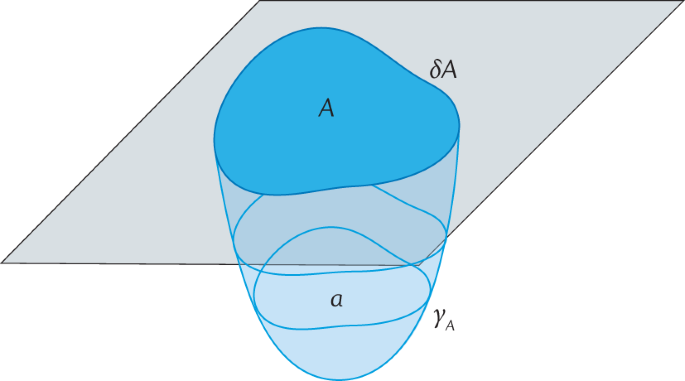
\includegraphics[width=0.2\textwidth]{../Imatges/Extern/EE_AdS-CFT.png}
\caption{Region $\calA$ (dark blue) and its boundary $\partial \calA$ inside a $z=\delta$ AdS slide (grey) and its respective $\gamma_{\calA}$ (light blue) inside the AdS spacetime.}
\label{fig:EE_AdS-CFT}
\end{wrapfigure}

The Ryu-Takayanagi formula is valid for generic systems, and gives a flavour of how the geometry of spacetime can emerge from mere quantum information. 

From the Ryu-Takayanagi formula for a ( $d+1$ )-dimensional anti-de Sitter spacetime one obtains the expected general expression of the entanglement entropy (Eq.~\ref{eq:EE}) for a $d$-dimensional conformal field theory \cite{}.

In the next subsection (Sec.~\ref{ss:EE-disk}) it is developed the procedure to compute the entanglement entropy for a circular region of a CFT$_3$.


\subsection{Entanglement Entropy for a Disk in CFT$_3$} \label{ss:EE-disk}

A circuilar region $\calA$ with radius $R$ inside a 2-dimensional layer $z = \delta \ll 1$ and the corresponding surface of minimal area $\delta_{\calA}$ are represented by polar coordinates as:
\eqgat{1A}{
    \calA = \{ ( r, \theta, z, t ) \ | \ t = 0, z = \delta, r \le R \} \nonumber \\
    \gamma_{\calA} = \{ ( r, \theta, z, t ) \ | \ t = 0, z = f (r, \theta) \} \ .
}
There is no property on the AdS spacetime theory that will make the symmetry of $\partial \calA$ on the coordinate $\theta$ not being transfered to $\gamma_{\calA}$. Hence, $z = f (r)$.

The metric corresponding to a ($d+1$)-dimensional AdS spacetime will be
\eq{1Ametric}{
    ds^2_{\text{AdS}_4} = g_{\mu \nu} dx^\mu dx^\nu = 
    \frac{L^2}{z^2} [ -dt^2 + dz^2 + dr^2 + r^2 d\theta^2 ] \ .
}

Applying the restrictions on the coordinates for the definition of $\gamma_{\calA}$, it is obtained the induced metric of the surface:
\eq{1gammaAmetric}{
    ds^2_{\gamma_{\calA}} = h_{\rho \sigma} dx^\rho dx^\sigma = 
    \frac{L^2}{f(r)^2} \left[ \left( 1+ \dot{f}(r)^2 \right) dr^2 + r^2 d\theta^2 \right] \ ,
}
being $dz = \partial_\rho z \ dx^\rho = \partial f(r)_r \ dr = \dot{f}(r) dr$.

The determinant of the induced metric will be
\eq{1h}{
    h = \left( \frac{L}{f(r)} \right) ^4 r^2 ( 1 + \dot{f}(r)^2 ) \ .
}

The minimal value of the integral over the polar coordinates of the square rood of the induced metric will correspond to the area of $\gamma_{\calA}$. So, by the Ryu-Takayanagi formula, the entanglement entropy related to the region $\calA$ will be
\eqgat{1EEA}{
    S_{\calA} = \frac{1}{4G} \text{min} \int_{\gamma_{\calA}} \sqrt{h} dx^\rho \nonumber \\
    = \frac{\pi L^2}{2G} \text{min} \int_0^R dr \frac{r}{f(r)^2} \sqrt{ 1 + \dot{f}(r)^2 } \ .
}

The interior of this final integral looks like some type of Lagrangian $\calL [r,f(r),\dot{f}(r)]$. Thus, the Euler-Lagrange equation can be aplied to find relations to find the extreme of this functional:
\eqgat{1EL}{
    \frac{\partial \calL}{\partial f} - \frac{d}{dr} \left[ \frac{\partial \calL}{\partial \dot{f}} \right] = 0 \nonumber \\
    \longrightarrow \left( 1+\dot{f}^2 \right) \left( -2r-f\dot{f}-rf\ddot{f} \right) + rf\dot{f}^2\ddot{f} = 0 \ .
}

One can prove that $f(r) = \sqrt{R^2 - r^2}$ is solution of the previous relation and corresponds to the function that minimise the functional of the entanglement entropy. Hence, the surface of minimal area is found to be a half sphere.

The entanglement entropy of the disk will be
\eq{1sol}{
    S_{\calA} = \frac{\pi L^2}{2G} \frac{R}{\delta} - F \ ,
}
that is equivalent to the general expression for the entanglement entropy in a 3-dimensional QFT.


\subsection{Strong subadditivity} \label{ss:SS}

The \textit{strong subadditivity} \cite{headrick_holographic_2007} defines relations between entanglement entropies of two subsystems $\calA$ and $\calB$, and its union $\calA \cup \calB$, interception $\cal \cap \calB$ and relative complement $\calA \setminus \calB$:
\eqgat{EE_strong-subadd}{
    S(\calA) + S(\calB) \ge S(\calA \cup \calB) + S(\calA \cap \calB) \ , \nonumber \\
    S(\calA) + S(\calB) \ge S(\calA \setminus \calB) + S(\calB \setminus \calA) \ .
}

\begin{wrapfigure}{r}{0.2\textwidth}
    \centering
    
\includegraphics[width=0.2\textwidth]{../Imatges/empty.png}
\caption{}
\label{fig:SS}
\end{wrapfigure}

This properties are present in any quantum mechanical many-body theory. An important test of the validity of the Ryu-Takayanagi formula (Eq.~\ref{eq:EE_RT}) is whether it fulfills this property.

Let's start proving the first inequality. Let $\gamma_{\calA}$, $\gamma_{\calB}$ be the surfaces of minimal area in the bulk connected to $\partial \calA$, $\partial \calB$ respectively, and $r_{\calA}$, $r_{\calB}$ the corresponding regions of the bulk (Fig.~\ref{fig:SS}). Thus, $\partial r_{\calA} = \calA \cup \gamma_{\calA}$, $\partial r_{\calB} = \calB \cup \gamma_{\calB}$, and we define the regions
\eq{SS_r-1}{
    r_{\calA \cup \calB} = r_{\calA} \cup r_{\calB} \ , \ r_{\calA \cap \calB} = r_{\calA} \cap r_{\calB} \ .
}
The surfaces onto the slice of these regions can be decomposed as
\eq{SS_dr-1}{
    \partial r_{\calA \cup \calB} = (\calA \cup \calB) \cup \gamma_{\calA \cup \calB} \ , \ \partial r_{\calA \cap \calB } = (\calA \cap \calB) \cup \gamma_{\calA \cap \calB} \ .
}
It is clear that $\partial (\calA \cup \calB)$ and $\partial (\calA \cap \calB)$ correspond to $\gamma_{\calA \cup \calB}$ and $\gamma_{\calA \cap \calB}$, but nothing says that they are the surfaces of minimal area $\gamma^{\text{min}}_{\calA \cup \calB}$ and $\gamma^{\text{min}}_{\calA \cap \calB}$ related to $\partial (\calA \cup \calB)$ and $\partial (\calA \cap \calB)$, they are upper bounds. This proves that
\eq{SS_gamma-1}{
    \gamma_{\calA} + \gamma_{\calB} = \gamma_{\calA \cup \calB} + \gamma_{\calA \cap \calB} \ge \gamma^{\text{min}}_{\calA \cup \calB} + \gamma^{\text{min}}_{\calA \cap \calB} \ ,
}
and, therefore, using the Ryu-Takayanagi formula (Eq.~\ref{eq:EE_RT}), the first inequality of Eq.~\ref{eq:EE_strong-subadd}.

Regarding the second inequality, we see that
\eq{SS_r-2}{
    r_{\calA \setminus \calB} = r_{\calA} \cup r_{\calB} \ , \ r_{\calB \setminus \calA} = r_{\calB} \cup r_{\calA} \ .
}
The surface onto the slice of these regions are decomposed as
\eq{SS_dr-2}{
    \partial r_{\calA \setminus \calB} = (\calA \setminus \calB) \cup \gamma_{\calA \setminus \calB} \ , \ \partial r_{\calB \setminus \calA } = (\calB \setminus \calA) \cup \gamma_{\calB \setminus \calA} \ .
}
The $\partial (\calA \setminus \calB)$ and $\partial (\calB \setminus \calA)$ correspond to the upper bounds $\gamma_{\calA \setminus \calB}$ and $\gamma_{\calB \setminus \calA}$ of the surfaces of minimal area $\gamma^{\text{min}}_{\calA \setminus \calB}$ and $\gamma^{\text{min}}_{\calA \setminus \calB}$. So
\eq{SS_gamma-2}{
    \gamma_{\calA} + \gamma_{\calB} = \gamma_{\calA \setminus \calB} + \gamma_{\calB \setminus \calA} \ge \gamma^{\text{min}}_{\calA \setminus \calB} + \gamma^{\text{min}}_{\calB \setminus \calA} \ ,
}
and, through the Ryu-Takayanagi formula, the second inequality of \ref{eq:EE_strong-subadd} it is proven.

Using this simple geometric proof, it is shown that holography fulfills the strong subadditivity property that should be true in any quantum mechanical many-body system, playing the extra dimension in the holographic dual an essential role.


\subsection{Entanglement entropy for higher orders} \label{s:EE_HO}





    
\newpage



\subsection{Entanglement entropy for higher orders} \label{s:EE_HO}

It has been shown that the Ryu-takayanagi formula (\ref{eq:EE_RT}) as the entanglement entropy for holographic theories dual to Einstein gravity. Nevertheless, working with effective actions makes higher-order terms appear as stringy and quantum corrections \cite{bueno_holographic_2021}.

For higher-curvature gravities (or stringy corrections), the area functional needs to be modified, similarly to how the Bekenstein-Hawking formula for the entropy of a black hole (\ref{eq:BH}) is replaced by Wald formula \cite{iyer_properties_1994}. But replacing the functional of the entanglement entropy for the Wald's one does not work \cite{bueno_holographic_2021}. Additional "anomaly" terms corresponding to extrinsic curvatures of the generalized surface involving arbitrary contractions of Riemann tensors and metrics are required \cite{dong_holographic_2014}. Schematically:
\eq{EE_HO}{
    S_{\text{HO}}(\calA) = S_{\text{Wald}} + S_{\text{Anomaly}} \ .
}

In the same way that one finds the entanglement entropy with the Ryu-Takayanagi formula (Sec.~\ref{ss:R-T}), the generalized holographic surface should be obtained by extremizing the new functional with the corrections of the previous expression. In the anomaly term, each of the Riemann tensor components resulting has to be split into summatories of different weighted terms. The way that these terms are weighted is non-unique, leading to the so-called \textit{splitting problem}.

One can also consider corrections on the Ryu-Takayanagi formula related to quantum mechanical effects in the bulk \cite{faulkner_quantum_2013}.

This quantum corrections are essentially given by the entanglement entropy between the bulk bounded by the minimal area surface and the outside region. One can see the bulk region as an effective field theory itself living on a fixed background geometry and compute its entanglement entropy as in any quantum field.

One has to be cautious and do not confuse this entanglement entropy with the one computed by the Ryu-Takayanagi formula, which is intended to be generalized.




\section{Duality with Einstein field equations} \label{s:EQ}

\subsection{First law of entanglement entropy} \label{ss:FLEE}

For a small perturbation of a quantum field theory state $\ket{\psi(\varepsilon)}$ to the initial state $\ket{\psi(0)}$, the \textit{First Law of Entanglement Entropy} is defined as
\eq{FLEE}{
    \delta S_{\calA} = \frac{d}{d \varepsilon} S_{\calA} = \frac{d}{d \varepsilon} \abs{H_{\calA}} = \frac{d}{d \varepsilon} \tr (H_{\calA} \rho_{\calA}) \equiv \delta E_{calA}
}
for the entanglement entropy of a subsystem $\calA$ \cite{fareghbal_first_2019}. The modular Hamiltonian $H_{\calA}$ is independent of the perturbation and is defined by
\eq{modularH}{
    \rho_{\calA} (\varepsilon) = e^{-H_{\calA}}.
}

The first law of entanglement entropy is a generalization of the first law of thermodynamics for any arbitrary small perturbation, quantum state or subsystem.

When $H_{\calA}$ is a local operator, $\rho_{\calA}$ can be mapped to a thermal one, $\rho_{\calH}$, by a unitary transformation, being the resultant entropy thermal. Hence, $\rho_{\calH}$ can be written as
\eq{modularH2}{
    \rho_{\calH} = \frac{e^{-H_{\calH}}}{\tr (e^{-H_{\calH}})} \ ,
}
where $H_{\calH}$ is the associated charge of the so-called modular flow $\xi$.

In the holographic description, it has been shown that writing both sites of the first law of entanglement entropy in terms of the corresponding bulk parameters leads to a constraint on the bulk geometry that is exactly the Einstein field equations \cite{fareghbal_first_2019}. If this was an intrinsic property of any gauge/gravity theory, one could use entanglement entropy in an arbitrary field theory to find a dual gravitational geometry.

\subsection{First law of entanglement entropy applied to holography} \label{ss:FLEE_H}

---

---

---




\section{Conclusions} \label{s:Conclusions}

---

the Ryu-Takayanagi formula in the case of a thermalized system of particles in an AdS space-time derives to the Bekenstein-Hawking formula \cite{bekenstein_black_1973} for the entropy a black hole:
\eq{BH}{
    S_{BH} = \frac{ A_H }{ 4 G } \ ,
}
that says that the entropy related to a black hole only depends on the area $A_H$ of its event horizon.

---

---




\begin{acknowledgments}
    ---
    
    ---
    
    ---
    
\end{acknowledgments}



\bibliography{TFG.bib}



\end{document}